\documentclass{book}
\usepackage[utf8]{vietnam}
\usepackage{cite}
\usepackage{amsmath,amssymb,amsfonts}
\usepackage{algorithm}
\usepackage{algorithmic}
\usepackage{graphicx}
\usepackage{textcomp}
\usepackage{xcolor}
\usepackage{tabularx}
\usepackage{listings}
\usepackage{enumerate}

\newcounter{savedenum}
\newcommand*{\saveenum}{\setcounter{savedenum}{\theenumi}}
\newcommand*{\resume}{\setcounter{enumi}{\thesavedenum}}


\begin{document}
%\title{TỐI ƯU LỒI VÀ ỨNG DỤNG TRONG MÁY HỌC}
%\author{Võ Thị Lưu Phương}
%
%
%\maketitle

\setcounter{chapter}{3}
\chapter{CÁC GIẢI THUẬT BẬC MỘT}
\textit{Tác giả: Võ Thị Lưu Phương\\Email: vtlphuong@hcmiu.edu.vn}

Không phải bài toán tối ưu nào cũng có nghiệm dạng công thức có thể tính trực tiếp được. 
Ngay cả bài toán tìm cực tiểu hàm toàn phương (quadratic) tuy có công thức nghiệm, nhưng việc tính nghiệm lại tốn nhiều tài nguyên, đăc biệt là khi bài toán có kích thước lớn. 
Do đó, các phương pháp được sử dụng phổ biến hiện nay để tìm nghiệm bài toán tối ưu lồi là sử dụng các giải thuật lặp cập nhật giá trị của các biến số nhiều lần để đạt tới giá trị tối ưu.

Trong chương này, ta xem xét các \emph{giải thuật bậc một} bao gồm gradient descent, schochastic gradient descent, subgradient và proximal gradient descent để giải một bài toán tối ưu lồi không có ràng buộc. 
Giải thuật bậc một có nghĩa là các cập nhật liên quan đến đạo hàm bậc một.

\section{DESCENT METHOD}

Xét bài toán tối ưu không có ràng buộc
\begin{align*}
\min_x f(x)
\end{align*}
trong đó $f$ là hàm lồi và khả vi tại mọi điểm trong miền xác định của $f$.

%Một số giải thuật trong chương này cần giả định hàm $f$ \emph{lồi chặt} (strongly convex).
%Hàm $f$ được gọi là lồi chặt nếu tồn tại số thực $m > 0$ sao cho
%\begin{align*}
%\nabla^2 f(x) \geq m I.
%\end{align*}
%(Nhắc lại, cho hai ma trận đối xứng $A, B$. Ta nói $A \geq B$ nếu $A-B$ là ma trân xác định dương.)
%
%Ta có, nếu $f$ lồi chặt thì tồn tại $z$ trên đoạn thẳng nối $[x,y]$ sao cho
%\begin{align*}
%f(y)  \geq f(x) + \|\nabla f(x)\|^T (y - x) + \frac{1}{2}  ( y-x)^T  \nabla^2 f(z) (y - x).
%\end{align*}
%Kết hợp với định nghĩa thì ta có 
%\begin{align*}
%f(y) \geq f(x) + \|\nabla f(x)\|^T (y - x) + \frac{m}{2} \| y-x \|_2^2
%\end{align*}
%cho mọi $x, y$ thuộc miền xác định.

Theo như bài trước thì điều kiện cần và đủ để $f$ đạt cực tiểu $x^*$ là
\begin{align*}
\nabla f(x^*) = 0.
\end{align*}
Giải thuật lặp sinh một dãy các điểm $x^{(0)}, x^{(1)}, \ldots , x^{(k)}, \ldots \in \mathbf{dom}f$ sao cho khi $k \rightarrow \infty$ thì $\nabla f(x^*) \rightarrow 0$ . 
Lúc đó, ta có $f(x^{(k)}) \rightarrow p^*$, là giá trị tối ưu.

%Về lý thuyết thì giải thuật bắt đầu từ điểm $x^{(0)}$ thỏa mãn
%\begin{itemize}
%\item $x^{(0)} \in \mathbf{dom}f$
%\item sublevel set $S = \{x | f(x) \leq f(x^{(0)})\}$ là tập đóng
%\end{itemize}


Cập nhật theo kiểu \textbf{giảm dần} có dạng tổng quát như sau
\begin{align*}
x^{(k+1)} = x^{(k)} + t_k \Delta x^{(k)}
\end{align*}
sao cho $f(x^{(k+1)}) < f(x^{(k)})$ được gọi chung là \emph{descent method}.
$\Delta x^{(k)}$ được gọi là \emph{search direction} và $t_k$ được gọi là \emph{line search}.

Từ điều kiện bậc một của hàm lồi, ta luôn có
\begin{align*}
f(y) \geq f(x) + \nabla f(x)^T (y - x).
\end{align*}
thay $y = x^{(k+1)}$ và $x = x^{(k)}$, ta có 
\begin{align*}
f(x^{(k+1)}) \geq f(x^{(k)}) + t_k \nabla f(x^{(k)})^T \Delta x^{(k)}.
\end{align*}
Để đảm bảo được tính giảm dần $f(x^{(k+1)}) < f(x^{(k)})$, ta bắt buộc phải có 
\begin{align}
\nabla f(x^{(k)})^T \Delta x^{(k)} <0.
\label{ep:descentcri}
\end{align}
Về mặt hình học thì vector $\nabla f(x^{k})$ và vector search direction $\Delta x^{k}$ phải tạo thành một \emph{góc tù}, hay nói cách khác, search direction và  vector $\nabla f(x)$ phải nằm khác halfspace được tạo bởi siêu phẳng $\nabla f(x^{k})^T (x - x^{k}) = 0$ (xem Hình \ref{fig:descent}).
\begin{figure}[h]
	\centering
	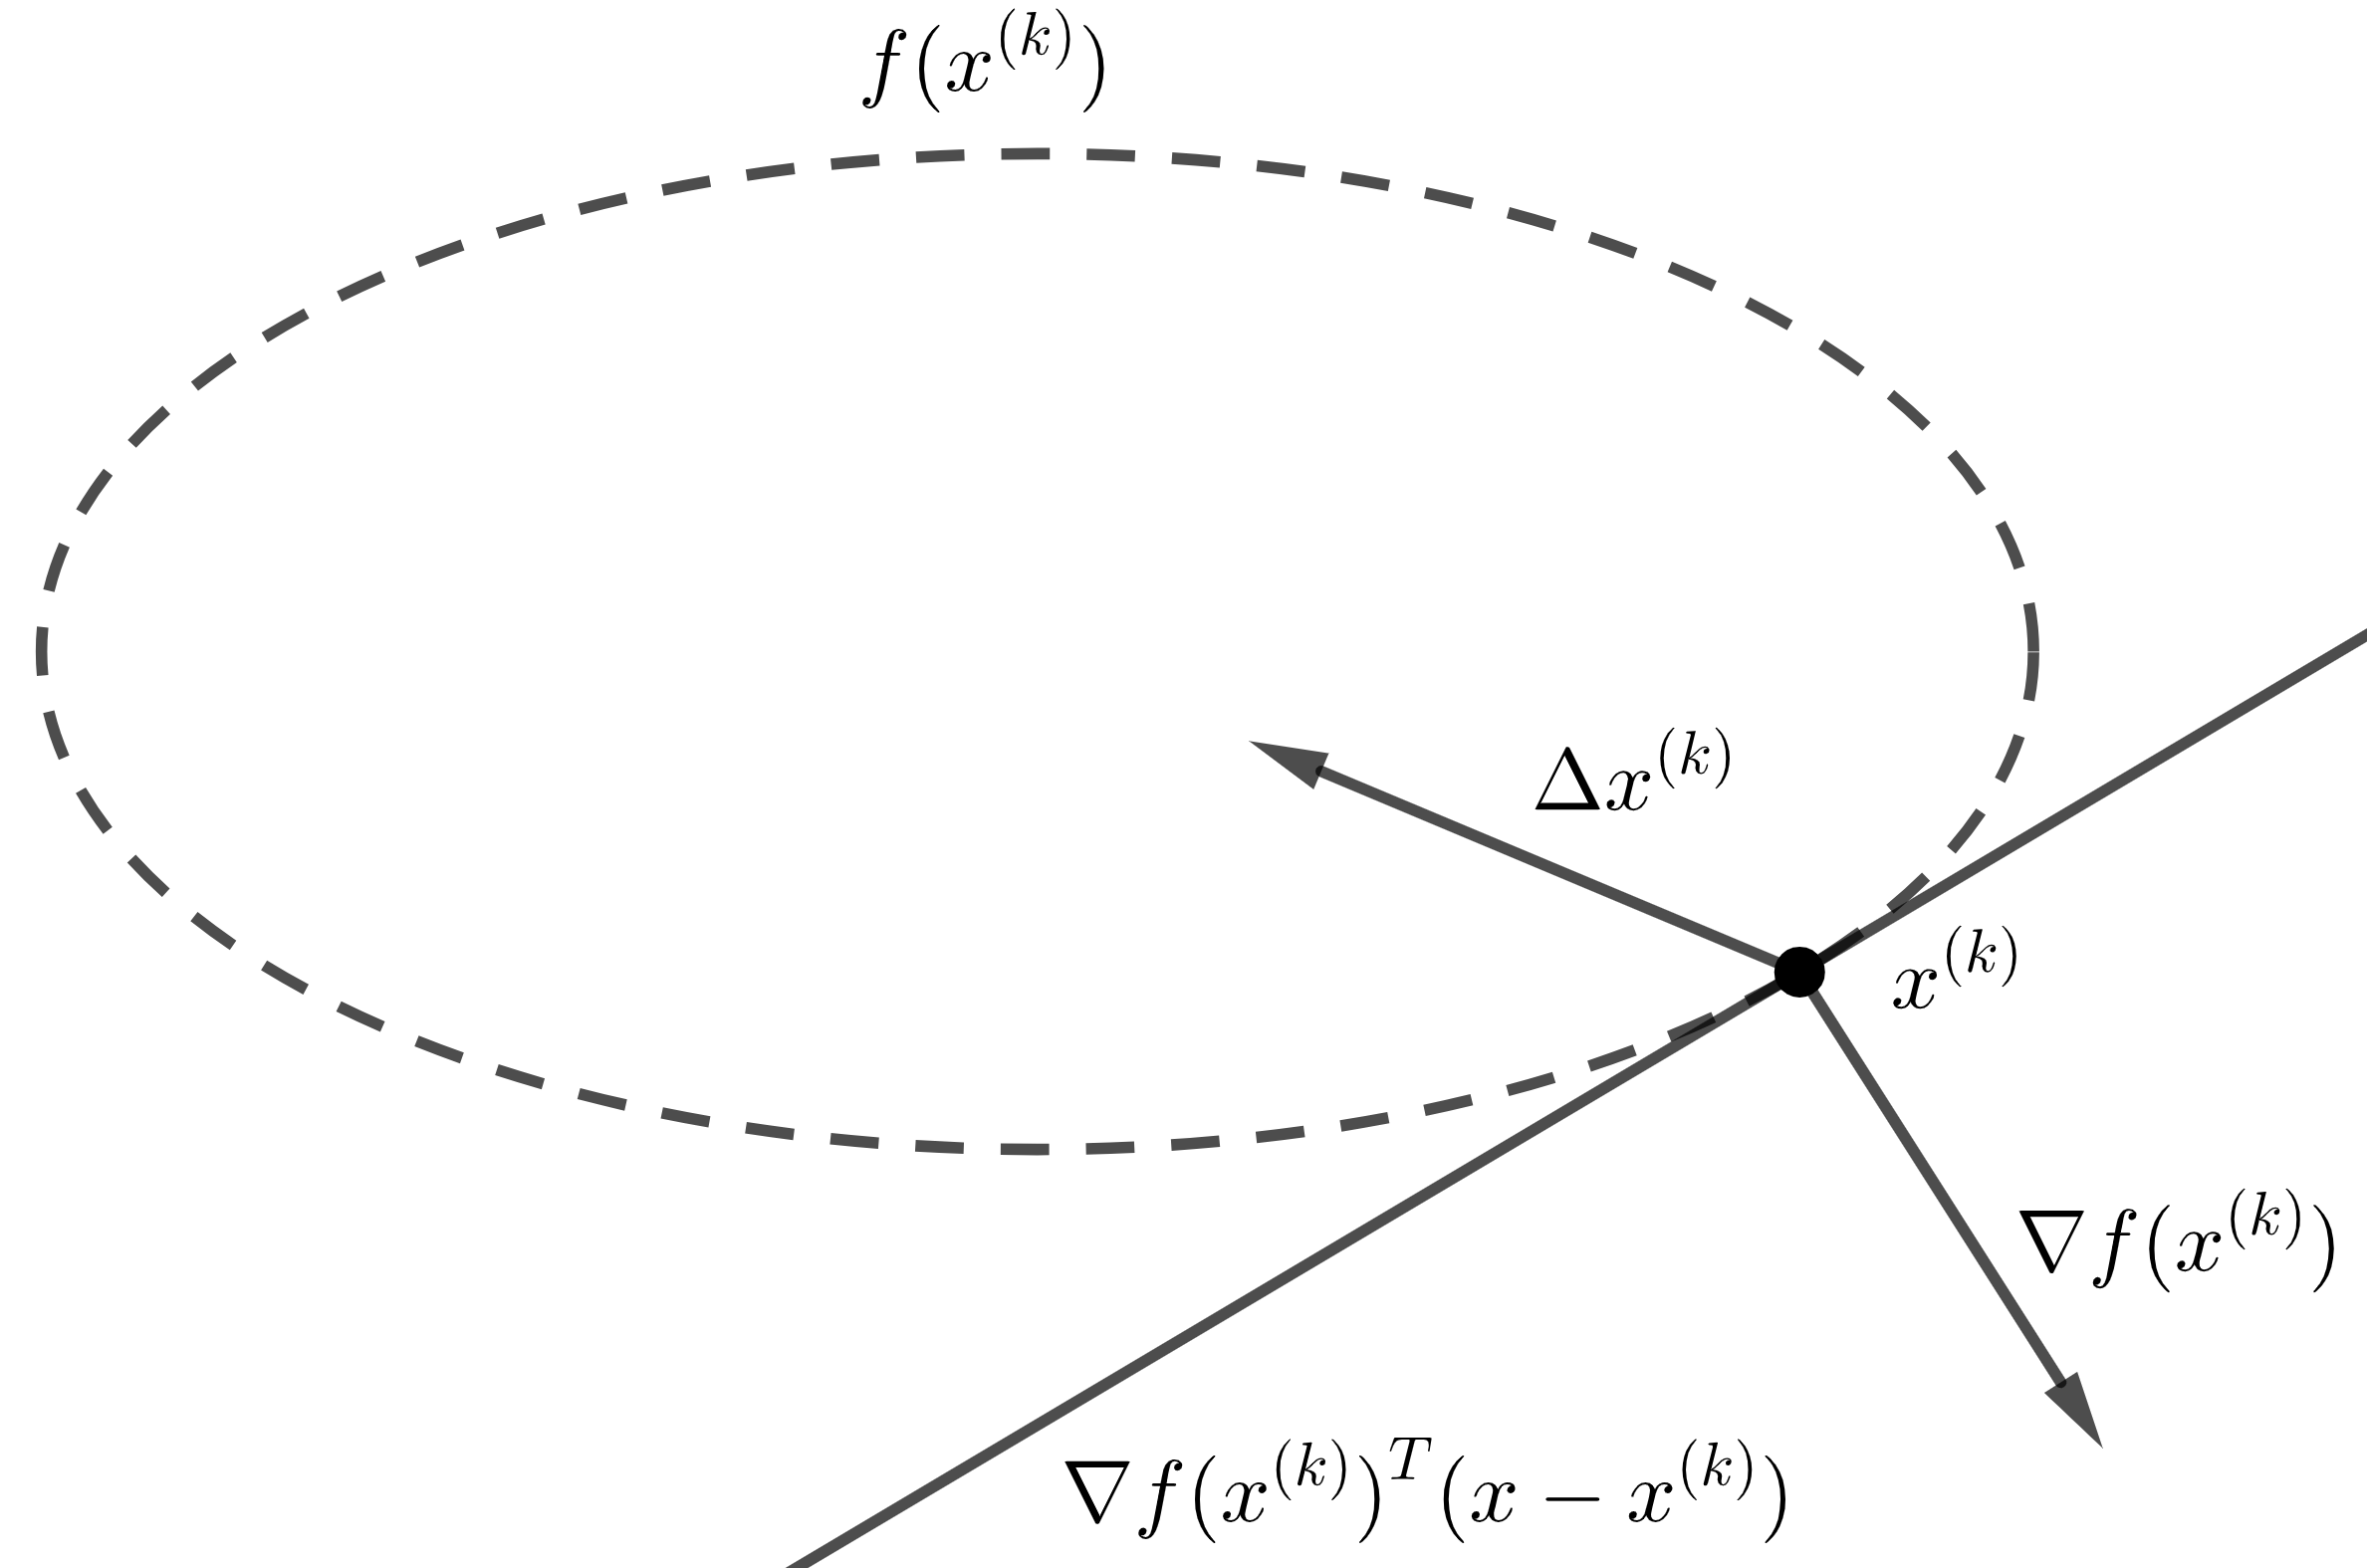
\includegraphics[width=8cm]{hinh_chuong4_algorithm/part5_descent.png}
	\caption{Minh họa của \emph{search direction} trong các phương pháp descent. Vector $\Delta x$ và vector $\nabla f(x)$ phải nằm ở hai nửa mặt phẳng khác nhau và tạo với nhau thành một góc tù.}
	\label{fig:descent}	
\end{figure}

Descent method tổng quát có dạng sau:
\begin{algorithm}[H]
%\begin{algorithmic}[1]
khởi tạo $x^{(0)} \in \mathbf{dom}f$;\\
\textbf{repeat} 
\begin{enumerate}
\item Xác định \emph{search direction} $\Delta x^{(k)}$;
\item \emph{Line search}: chọn step size $t_k >0$.
\item Cập nhật: $x^{(k+1)} = x^{(k)} + t_k \Delta x^{(k)}$, $k=1,2,3...$
\end{enumerate}
\textbf{until} hội tụ. 
\caption{Descent method dạng tổng quát.}
\label{alg:descent}
%\end{algorithmic}
\end{algorithm}
Giải thuật được xem là hội tụ nếu điều kiện dừng (stopping criterion) thỏa mãn. Về lý thuyết, điều kiện dừng là $\|\nabla f(x)\|_2 \leq \epsilon$, trong đó $\epsilon$ là một số dương đủ nhỏ.

Step size trong mỗi vòng lặp được tính bởi:
\begin{itemize}
\item \emph{exact line search}: trong cách này, step size $t$ được chọn sao cho giá trị hàm số giảm nhiều nhất trong mỗi vòng lặp:
\begin{align*}
t = \mathrm{argmin}_{t>0} f(x + t \Delta x)
\end{align*}

\item \emph{backtracking line search} với $\alpha \in (0, 1/2)$, $\beta \in (0, 1)$ và khỏi tạo $t = 1$,\\
lặp lại $t:= \beta t$ cho đến khi $f(x + t \Delta x)  \leq f(x) + \alpha t \nabla f(x)^T \Delta x$ thì ngưng.
%\item graphical interpretation: backtrack until $t \leq t_0$
\end{itemize}
\emph{Exact line search} không hiệu quả trong phần lớn các bài toán vì cần phải giải một bài toán tối ưu $\mathrm{min}_{t>0} f(x + t \Delta x)$ trong mỗi vòng lặp. 
Tuy nhiên trong một số bài toán đặc biệt mà nghiệm $\mathrm{argmin}_{t>0} f(x + t \Delta x)$ có thể được tính ra dạng công thức, ta cũng có thể dùng exact line search.

\subsection{Phương pháp gradient descent (GD)}
Phương pháp \emph{gradient descent} (GD) chọn search direction $\Delta x$ chính bằng $-\nabla f(x)$. Do đó giải thuật gradient descent có dạng sau:
\begin{algorithm}[H]
%\begin{algorithmic}[1]
khởi tạo $x^{(0)} \in \mathbf{dom}f$;\\
\textbf{repeat} 
\begin{enumerate}
\item \emph{Line search}: chọn step size $t_k$.
\item Cập nhật: $x^{(k+1)} = x^{(k)} - t_k \nabla f(x^{(k)})$, $k=1,2,...$
\end{enumerate}
\textbf{until} hội tụ. 
\caption{Giải thuật gradient descent.}
\label{alg:gd}
%\end{algorithmic}
\end{algorithm}

Về lý thuyết, giải thuật được xem là hội tụ khi vector gradient đủ nhỏ: $\| \nabla f(x) \|_2 \leq \epsilon$.
Tuy nhiên, trong thực tế ta thường cho chạy một số vòng lặp nhất định và quan sát sự hội tụ qua đồ thị, qua chuỗi số $x$. Một cách khác là dừng khi khoảng cách giữa hai giá trị liên tiếp đủ nhỏ $\|x^{(k)} - x^{(k-1)}\|_2 \leq \epsilon$.

\subsubsection*{Tính chất hội tụ của GD}
Đầu tiên ta cần định nghĩa về điều kiện \emph{Lipschitz continuous} thường cần cho sự hội tụ của giải thuật.
Một hàm số $f$ được gọi là \emph{Lipschitz continuous} nếu tồn tại số thực dương $L$ sao cho
\begin{align}
\|f(x) - f(y) \|_2 \leq L \|x-y\|_2.
\end{align}
Điều kiện \emph{Lipschitz continuous} giới hạn sự thay đổi quá nhanh của hàm số.

Nếu $f$ là hàm lồi, khả vi và $\nabla f$ là $L$-Lipschitz continuous, phương pháp GD với \emph{step size hằng số $t \leq 1/L$} hội tụ. Cụ thể là,
\begin{align*}
f(x^{(k)}) - p^* \leq \frac{\|x^{(0)} - p^*\|^2_2}{2tk} = \frac{C}{k},
\end{align*}
trong đó $C$ là một hằng số.
Do đó, \emph{GD hội tụ về cực tiểu với tốc độ hội tụ là $O(1/k)$}, hội tụ theo hàm tuyến tính.

Nếu ta đặt điều kiện $\frac{\|x^{(0)} - p^*\|^2_2}{2tk} \leq \epsilon$, với $\epsilon$ đủ nhỏ thì 
\begin{align*}
k \geq \frac{\|x^{(0)} - p^*\|^2_2}{2t \epsilon} = \frac{C}{k}.
\end{align*}
Do đó ta còn gọi tốc độ hội tụ của GD là $O(1/\epsilon)$.

Nếu ta có thêm điều kiện mạnh hơn: hàm $f$ lồi chặt (strongly convex), tức là tồn tại số thực dương $m$ sao cho $f(x) - \frac{m}{2}\|x\|^2_2$ là hàm lồi, 
thì giải thuật GD với step size hằng số $t \leq 2/(m+L)$ hoặc với backtracking line search có tính chất
\begin{align*}
f(x^{(k)}) - p^* \leq c^k \frac{L}{2}\|x^{(0)}) - p^*\|^2_2,
\end{align*}
trong đó $c$ là hằng số, $0 <c<1$ chỉ tùy thuộc vào $m$, $x^{(0)}$.
Do đó tốc độ hội tụ của GD trong trường hợp này là $O(c^k)$ hay còn gọi $O(\log(1/\epsilon))$, hội tụ theo hàm mũ.

%\textcolor{blue}{Blue} point is $x$, \textcolor{red}{red} point is $x = \mathrm{argmin}_y f(x) + \nabla f(x)^T (y - x) + \frac{1}{2t} \|y -x\|_2^2$ 

Trong thực tế thì ta khó biết được các hằng số $L$ hay $m$, do đó nếu chọn step size là hằng số, thì thường thử một vài lần và chọn step size $t$ đủ nhỏ phù hợp. Nếu $t$ lớn thì giải thuật không hội tụ. Còn nếu $t$ nhỏ quá thì giải thuật hội tụ chậm.

%Nếu dùng \emph{backtracking line search} thì xác định step size cho mỗi vòng lặp như sau:
%\begin{itemize}
%\item chọn $0 < \beta < 1$ and $0 < \alpha \leq 1/2$
%\item khởi tạo $t = t_{init}$, 
%\item nếu
%\begin{align*}
%f(x - t \nabla f(x)) > f(x) - \alpha t \| \nabla f(x)\|_2^2
%\end{align*}
%thì giảm $t = \beta t$. 
%\item nếu điệu kiện trên không thỏa thì cập nhật GD
%\begin{align*}
%x := x - t \nabla f(x).
%\end{align*}
%\end{itemize}

\subsection{Gradient descent áp dụng một số bài toán cụ thể}
\subsubsection{Giải thuật GD áp dụng cho linear regression}
Bài toán hồi quy tuyến tính với hàm sai số là $\ell_2$-norm được cho bởi
\begin{align}
\mathrm{min.} ~ L(w) = \sum_{i=1}^N (y_i - x_i^Tw)^2 = ||y - Xw||_2^2.
\end{align}
Trong đó $X = \begin{bmatrix} x_1^T \\ ... \\ x_{N}^T\end{bmatrix}$ và $y = \begin{bmatrix} y_1 \\ ... \\ y_{N}\end{bmatrix}$.
(Vui lòng tham khảo bài ``Linear regession'' để biết cách mô hình hóa dưới dạng một bài toán tối ưu.)

Do đó gradient có dạng
\begin{align*}
\nabla L(w) =  2 \sum_{i=1}^N x_i (x_i^T w - y_i) = 2(X^T X w - X^T y)
\end{align*}

Gradient descent áp dụng cho least square:
\begin{algorithm}[H]
%\begin{algorithmic}[1]
khởi tạo $w$;\\
\textbf{repeat} 
\begin{enumerate}
\item chọn step size $t$.
\item Cập nhật: 
\begin{align*}
w := w - 2t \sum_{i=1}^N x_i (x_i^T w - y_i)
\end{align*}
hay theo dạng ma trận
\begin{align*}
w := w - 2t (X^T X w - X^T y)
\end{align*}
\end{enumerate}
\textbf{until} giải thuật hội tụ. 
\caption{Giải thuật gradient descent áp dụng cho least square.}
\label{alg:gd_leastsquare}
%\end{algorithmic}
\end{algorithm}

Lưu ý, nếu sai số có dạng $\ell_1$-norm thì không áp dụng được giải thuật gradient vì đây không phải là hàm khả vi.

\subsubsection{Giải thuật GD áp dụng cho logistic regression}
Bài toán phân hai lớp logistic regression có dạng như sau:
\begin{align*}
\mathrm{max.} J(w) = \sum_{i=1}^N J_i(w) = \sum_{i=1}^N y_i x_i^T w - \log (1 + e^{ x_i^T w}),
\end{align*}
trong đó $x_i, y_i$ là vector đặc tính và nhãn của mẫu dữ liệu thứ $i$. 
(Xem logistic regression trong phần ứng dụng.)

Ta có gradient
\begin{align*}
J_i(w) & = y_i x_i - \frac{e^{x_i^T w}}{1 + e^{x_i^T w}} * x_i \\
		& = (y_i - \sigma_i)x_i,
\end{align*}
trong đó  $\sigma_i = \frac{e^{x_i^T w}}{1 + e^{x_i^T w}}$.
 
Giải thuật gradient descent áp dụng cho logistic regression có dạng như sau:
\begin{algorithm}[H]
%\begin{algorithmic}[1]
khởi tạo $w$;\\
\textbf{repeat} 
\begin{enumerate}
\item chọn step size $t$.
\item Cập nhật: 
\begin{align*}
w := w + t \sum_{i=1}^N (y_i - \sigma_i)x_i
\end{align*}
\end{enumerate}
\textbf{until} hội tụ. 
\caption{Giải thuật gradient descent áp dụng cho logistic regression.}
\label{alg:gd_logistic}
%\end{algorithmic}
\end{algorithm}
\textbf{Lưu ý}, bài toán tối ưu là bài toán tìm cực đại hàm lõm, do đó cập nhật phải có dạng
\begin{align}
w := w + t \nabla J(w).
\label{eq:grad_ascent}
\end{align}
Nhiều tài liệu gọi giải thuật trên là \textbf{gradient ascent}. Tuy nhiên tôi vẫn giữ nguyên tên gradient descent vì gradient ascent được suy ra trực tiếp từ gradient descent. 



\begin{figure}[h]
	\centering
	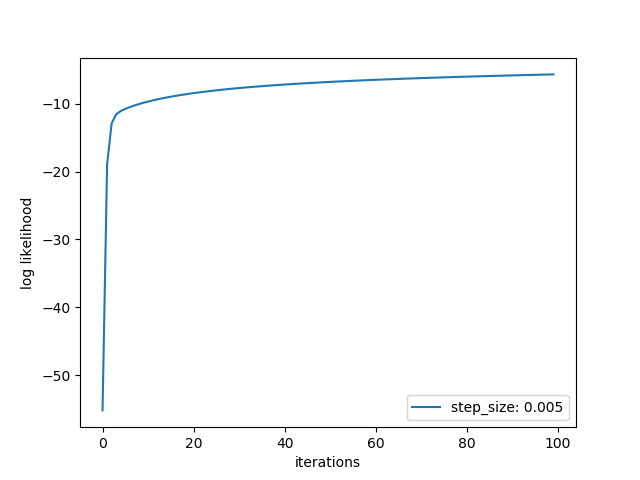
\includegraphics[width=8cm]{hinh_chuong4_algorithm/logistic-regression_synthetic_GD_obj_s0.005}
	\caption{Giải thuật không hội tụ với \lstinline{step_size = 0.005}.}
	\label{fig:descent}	
\end{figure}

\begin{figure}[h]
	\centering
	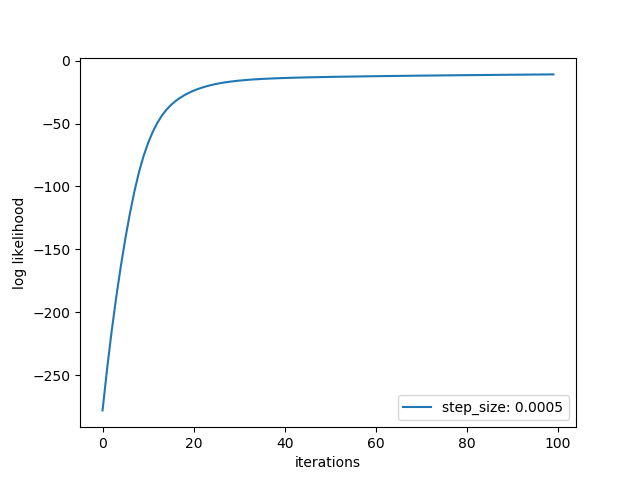
\includegraphics[width=8cm]{hinh_chuong4_algorithm/logistic-regression_synthetic_GD_obj_s0.0005.png}
	\caption{Giải thuật hội tụ với \lstinline{step_size = 0.0005}.}
	\label{fig:descent}	
\end{figure}


\newpage
\section{STOCHASTIC GRADIENT DESCENT METHOD (SGD)}
Trong gradient descent (GD), mỗi lần lặp là giải thuật tính gradient của $f(x)$ để thực hiện cập nhật. 
Tuy nhiên đối với những tập dữ liệu lớn, nhiều điểm dữ liệu thì vector gradient cũng rất lớn. Từ đó dẫn đến cập nhật mỗi vòng lặp của GD có độ phức tạp tính toán cao. 
Đối với bài toán có hàm mục tiêu dạng trung bình cộng các hàm số, ta có thể áp dụng phương pháp stochastic gradient descent (SGD) để hạn chế được nhược điểm của GD.

Xét bài toán tối ưu có hàm mục tiêu như sau
\begin{align*}
\min_x \frac{1}{m}\sum_{i=1}^m f_i (x).
\end{align*}
Dạng hàm số này xuất hiện nhiều trong học máy như linear regression, logistic regression.

Vì gradient $\nabla \sum_{i=1}^m f_i(x) =  \sum_{i=1}^m \nabla f_i(x)$, nên cập nhật trong mỗi vòng lặp của GD có dạng:
\begin{align*}
x^{(k)} = x^{(k-1)} - t_k  \frac{1}{m}\sum_{i=1}^m \nabla f_i (x^{(k-1)}), \quad k=1,2,\ldots.
\end{align*}

Trong SGD, ta xem $\nabla f_i (x^{(k-1)})$ là một xấp xỉ của mean của các gradient của $f_i$
\begin{align*}
\nabla f_i(x) \approx \mathbb{E}[\nabla f_{i_k} (x)].
\end{align*}
Do đó, cập nhật được thay thế như sau:
\begin{align}
x^{(k)} = x^{(k-1)} - t_k  \nabla f_{i_k} (x^{(k-1)}), \quad k=1,2,\ldots,
\label{eq:update_sgd}
\end{align}
trong đó $i_k \in \{1, 2, \ldots, m\}$ là index được chọn trong vòng lặp $k$.
\emph{Do cập nhật trong SGD chỉ liên quan đến một hàm $\nabla f_{i_k} (x^{(k-1)})$, nên độ phức tạp của mỗi cập nhật là thấp hơn hẳn GD và độc lập với độ lớn của $m$.} 

Ta có thể lựa chọn index $i_k$ trong vòng lặp $k$ bằng cách:
\begin{itemize}
\item Chọn \emph{ngẫu nhiên} theo uniform $i_k \in \{1, 2, \ldots, m\}$, hay
\item Chọn \emph{tuần tự} $i_k = 1, 2, \ldots, m, 1, 2, \ldots, m, \ldots$
\end{itemize}
Chọn ngẫu nhiên khá thông dụng trong thực tế. Khi chọn ngẫu nhiên, $\nabla f_{i_k} (x)$ chính là một mẫu ngẫu nhiên của gradient.

\subsection{Hội tụ của SGD}
Step size hằng số không làm cho SGD hội tụ. Về lý thuyết thì step size cho SGD phải là \textbf{diminishing step size}.
Diminishing step sizes thỏa các điều kiện sau:
\begin{align*}
\sum_{k=1}^{\infty} t_k^2 < \infty, \quad \sum_{k=1}^{\infty} t_k =\infty,
\end{align*}
tổng thì không có giới hạn, nhưng tổng bình phương thì có giới hạn. Hay nói một cách trực quan, dãy số step size tiến tới 0, nhưng không quá nhanh.  
Một ví dụ của diminishing step size $t_k = 1/k$.

Giả sử hàm $f$ lồi và giải thuật SGD dùng diminishing step size, ta có
\begin{align*}
\mathbb{E}[ f(x^{(k)})] - f^* = O(1 / \sqrt{k}).
\end{align*}
Tốc độ hội tụ là $1/\sqrt{k}$.


\subsection{SGD dùng mini-batch}
Một phương pháp phổ biến hiện nay là SGD dùng mini-batch.
Trong mỗi vòng lặp $k$, chọn một tập ngẫu nhiên  $\mathcal{B}_k \subseteq \{1, \ldots, m\}$ với kích thước $|\mathcal{B}_k| = B$ rất nhỏ hơn so với $m$. $B$ được gọi là batch size. Cập nhật trong vòng lặp $k$ có dạng
\begin{align*}
x^{(k)} = x^{(k-1)} - t_k \frac{1}{B} \sum_{i \in \mathcal{B}_k} \nabla f_{i} (x^{(k-1)}), \quad k=1,2,\ldots.
\end{align*}
Như vậy trong cập nhật trên, ta dùng $\frac{1}{B} \sum_{i \in \mathcal{B}_k} \nabla f_{i} (x^{(k-1)})$ thay cho gradient $\nabla f(x) = \frac{1}{m} \sum_{i \in m} \nabla f_{i} (x^{(k-1)})$.

Khi batch size lớn thì độ giao động của SGD nhỏ. Tuy nhiên độ phức tạp trong một cập nhật lại tăng lên. 


%So sánh giữa các phương pháp:
%\begin{itemize}
%\item One batch update costs $O(np)$
%\item One mini-batch update costs $O(bp)$
%\item One stochastic update costs $O(p)$
%\end{itemize}


\subsection{Ví dụ áp dụng SGD trong logistic regression}
Theo như bài trước, bài toán tối ưu cho logistic regression trong binary classification được viết dưới dạng
\begin{align*}
\max_{w} \frac{1}{N} \sum_{i = 1}^N \Big( y_i x_i^T w - \log (1 + e^{x_i^T w}) \Big)
\end{align*}

Hàm mục tiêu có dạng $f(w) =  \frac{1}{N} \sum_{i = 1}^n f_i(w)$, trong đó
\begin{align*}
f_i(w) =  y_i x_i^T w - \log (1 + e^{x_i^T w}).
\end{align*}

Ta có
\begin{align*}
\nabla f_i(w) =  y_i x_i - \frac{x_i e^{x_i^T w}}{1 + e^{x_i^T w}} = x_i(y_i - \sigma(x_i^T w)).
\end{align*}

Vậy SGD áp dụng cho logistic regression có dạng:
\begin{algorithm}[H]
%\begin{algorithmic}[1]
khởi tạo $w$;\\
\textbf{repeat} 
\begin{enumerate}
\item chọn step size $t$;
\item chọn ngẫu nhiên một mẫu dữ liệu $x_i, y_i$;
\item cập nhật: 
\begin{equation}
w := w + t x_i(y_i - \sigma(x_i^T w));
\label{eq:SGD_logistic}
\end{equation}
\end{enumerate}
\textbf{until} giải thuật hội tụ. 
\caption{Giải thuật SGD áp dụng cho logistic regression.}
\label{alg:batchSGD_logistic}
%\end{algorithmic}
\end{algorithm}

Trong trường hợp thực hiện mini-batch SGD, giải thuật có dạng sau:
\begin{algorithm}[H]
%\begin{algorithmic}[1]
khởi tạo $w$;\\
\textbf{repeat} 
\begin{enumerate}
\item chọn step size $t$;
\item chọn một batch gồm $B$ mẫu dữ liệu ngẫu nhiên;
\item cập nhật: 
\begin{equation}
w := w + \frac{t}{B} \sum_{i=1}^B x_i(y_i - \sigma(x_i^T w));
\label{eq:batchSGD_logistic}
\end{equation}
\end{enumerate}
\textbf{until} giải thuật hội tụ. 
\caption{Giải thuật SGD áp dụng cho logistic regression.}
\label{alg:batchSGD_logistic}
%\end{algorithmic}
\end{algorithm}

\textbf{SGD là một trường hợp đặc biệt của mini-batch SGD với batch size là 1.} 



\begin{figure}[h]
	\centering
	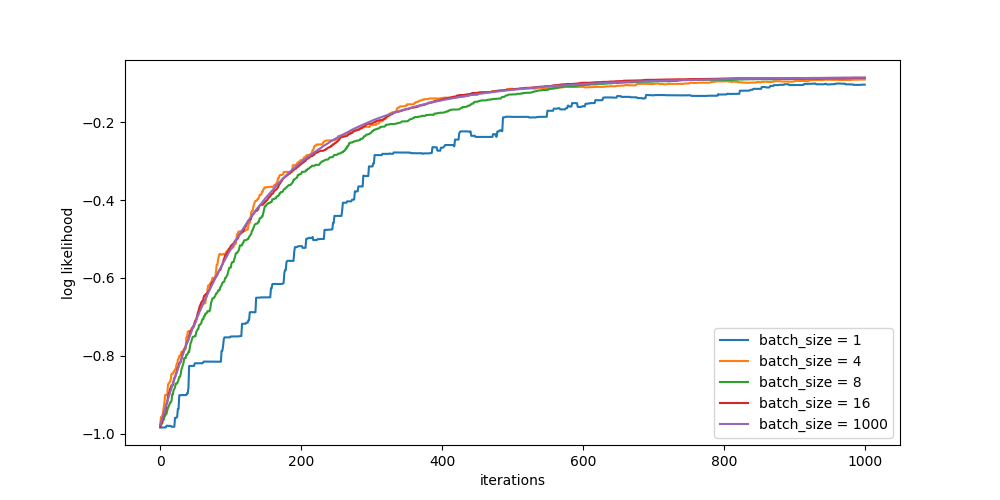
\includegraphics[width=10cm]{hinh_chuong4_algorithm/part5_logistic-regression_synthetic_stochasticGD_s0.005.png}
	\caption{Giải thuật mini-batch SGD với các batch size khác nhau.}
	\label{fig:descent}	
\end{figure}

Ta nhận thấy theo hình trên, chỉ với batch size khá nhỏ, giải thuật đã hội tụ khá tốt, tiệm cận với GD.

\newpage

\section{SUB-GRADIENT METHOD}
Giải thuật gradient descent yêu cầu hàm mục tiêu $f$ phải khả vi tại mọi điểm. Tuy nhiên, có một số hàm không thỏa điều kiện này ví dụ tối ưu hàm số $f$ có thêm $\ell_1$-norm regularization, nên không thể áp dụng gradient descent. Phương pháp subgradient có thể sử dụng cho bài toán này.

\subsection{Subgradient}

Hàm $g$ là một subgradient of $f$ tại điểm $x$ nếu
\begin{align*}
f(y) \geq f(x) + g^T(y - x) \quad \forall y
\end{align*}
\begin{figure}
\centering
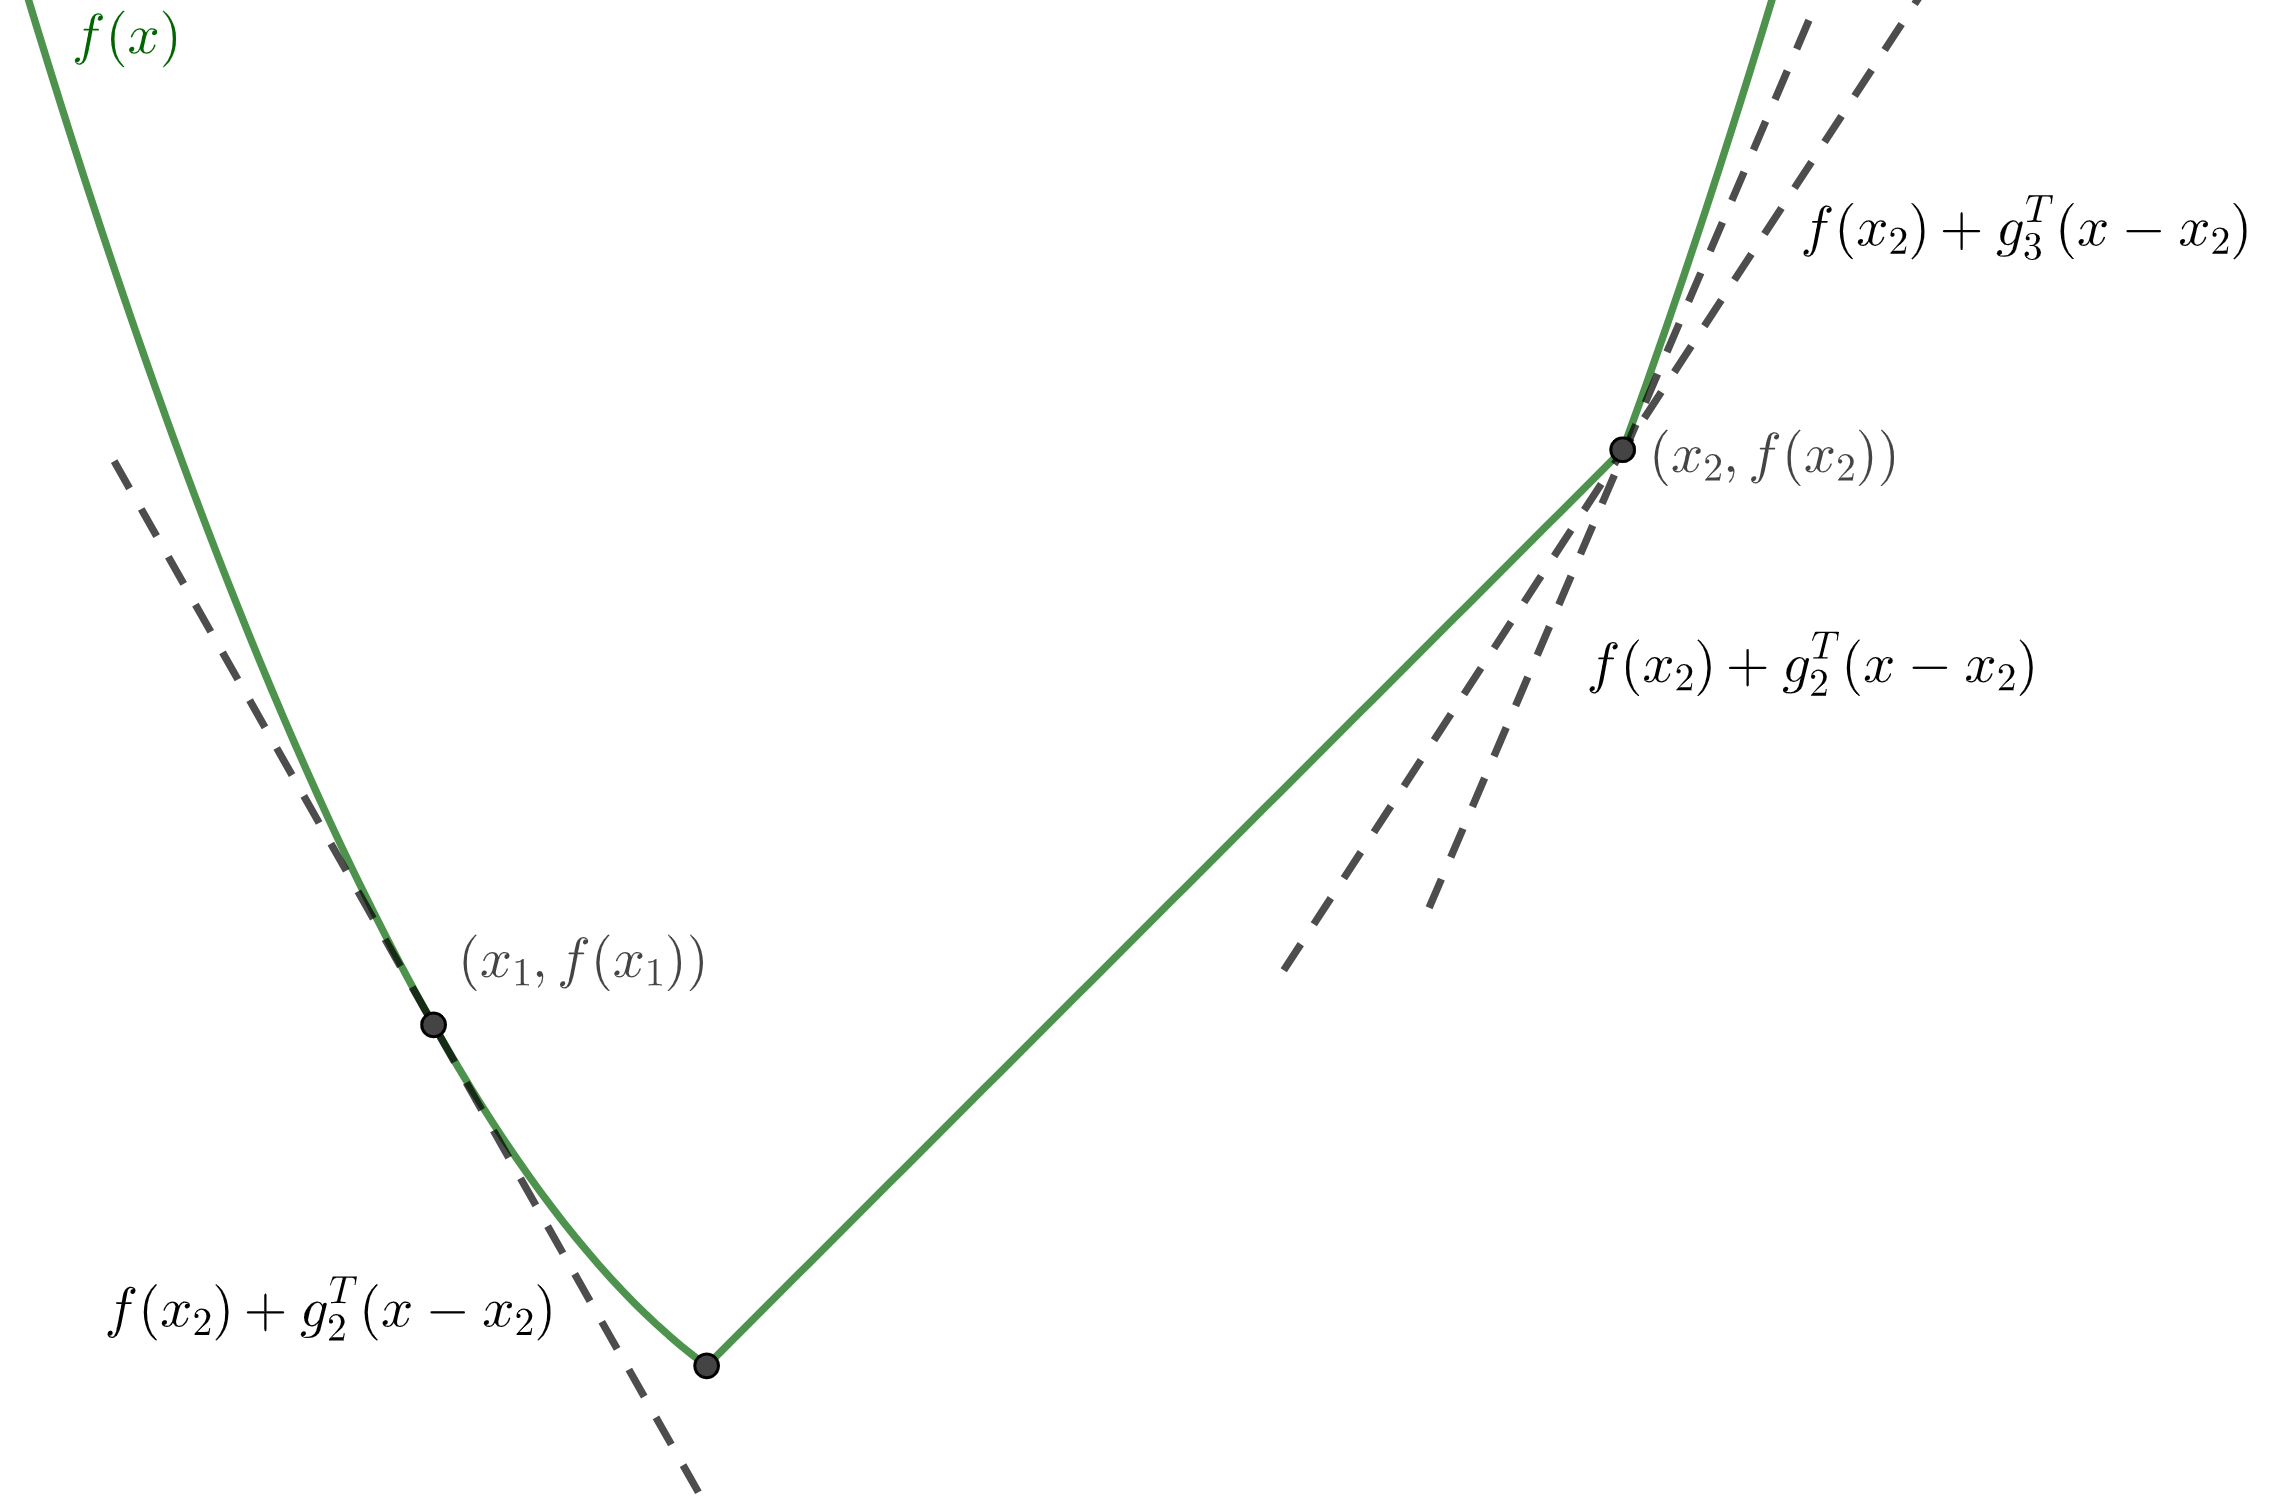
\includegraphics[width=8cm]{hinh_chuong4_algorithm/part5_subgradient.png}
\caption{Subgradient là duy nhất tại điểm $x_1$ khả vi. Hàm số có thể có nhiều subgradient tại điểm $x_2$ không khả vi.}
\end{figure}

Như vậy, ta thấy nếu $f$ lồi và khả vi thì gradient cũng chính là một subgradient tại $x$.

Tập hợp các subgradient của hàm $f$ thì được gọi là \textbf{subdifferential}, ký hiệu là $\partial f(x)$.
Ta có nếu hàm $f$ lồi thì subdifferential luôn tồn tại và có giới hạn. 
Nếu $f$ khả vi thì tại $x$, thì $\partial f(x) = \{\nabla f(x) \}$.
Ngược lại, nếu $\partial f(x) = \{ g \}$, thì $f$ khả vi tại $x$ và $g = \{\nabla f(x) \}$. 


\subsubsection{Các tính chất của subgradient}
Một số tính chất sau giúp tính subgradient của một hàm số:
\begin{itemize}
\item Nhân với một hằng số: $\partial(af) = a* \partial f$ với $a >0$
\item Cộng: $\partial(f_1 + f_2) = \partial f_1 + \partial f_2$
\item Kết hợp tuyến tính: nếu $g(x) = f(Ax + b)$, thì 
\begin{align*}
\partial g(x) = A^T \partial f(Ax + b)
\end{align*}
\item $f(x) = \max_{i = 1, \ldots, m} f_i(x)$: tại điểm $x$, hàm $f_i(x)$ làm lớn nhất thì subgradient chính là của $f$ chính là $\partial f_i(x)$.
Theo lý lý thuyết thì:
\begin{align*}
\partial f(x) = \mathrm{conv} (\cup_{i:f(x) = f_i(x)} \partial f_i(x)).
\end{align*}
\end{itemize}

\subsubsection{Một số ví dụ}
Một số ví dụ về subgradient của các hàm số:
\begin{itemize}
\item Hàm $f(x) = |x|, x \in \mathbf{R}$, có subgradient duy nhất $\mathrm{sign}(x)$ tại bất cứ điểm nào thỏa $x \neq 0$ ($\mathrm{sign}(x) = 1$ nếu $x>0$, $-1$ nếu $x<0$). Tại $x = 0$, subgradient là bất cứ giá trị nào thuộc $[-1, 1]$.
\item Hàm $f(x) = \|x \|_1, x \in \mathbf{R}^n$
\begin{align}
g_i = \begin{cases} \mathrm{sign}(x)  \textrm{ nếu } x_i \neq 0\\
				 \textrm{ bất cứ giá trị nào thuộc } [-1,1] \textrm{ nếu } x_i = 0.
\end{cases}
\label{eq:subgradient-norm1}
\end{align}
\item Hàm $f(x) = \|x \|_2, x \in \mathbf{R}^n$ có subgradient 
duy nhất $x / \|x \|_2$ tại $x \neq 0$. Tại $x =0$, subgradient là bất cứ giá trị nào thỏa $\{ z: \| z \|_2 \leq 1 \}$.
\item Hàm $f(x) = \max\{f_1(x), f_2(x)\}$, với $x \in \mathbf{R}^n$, $f_1, f_2$ là các hàm lồi và khả vi có subgradient 
\begin{align}
g = \begin{cases} \nabla f_1(x), \textrm{ nếu } f_1 (x) > f_2(x)\\
				\nabla f_2(x), \textrm{ nếu } f_1 (x) < f_2(x)\\
				\alpha \nabla f_1(x) + (1-\alpha)\nabla f_2(x), \forall \alpha \in [0,1], \textrm{ nếu } f_1 (x) = f_2(x).
\end{cases}
\label{eq:subgradient-piecewiselinear}
\end{align}
\end{itemize}

\begin{figure}
\centering
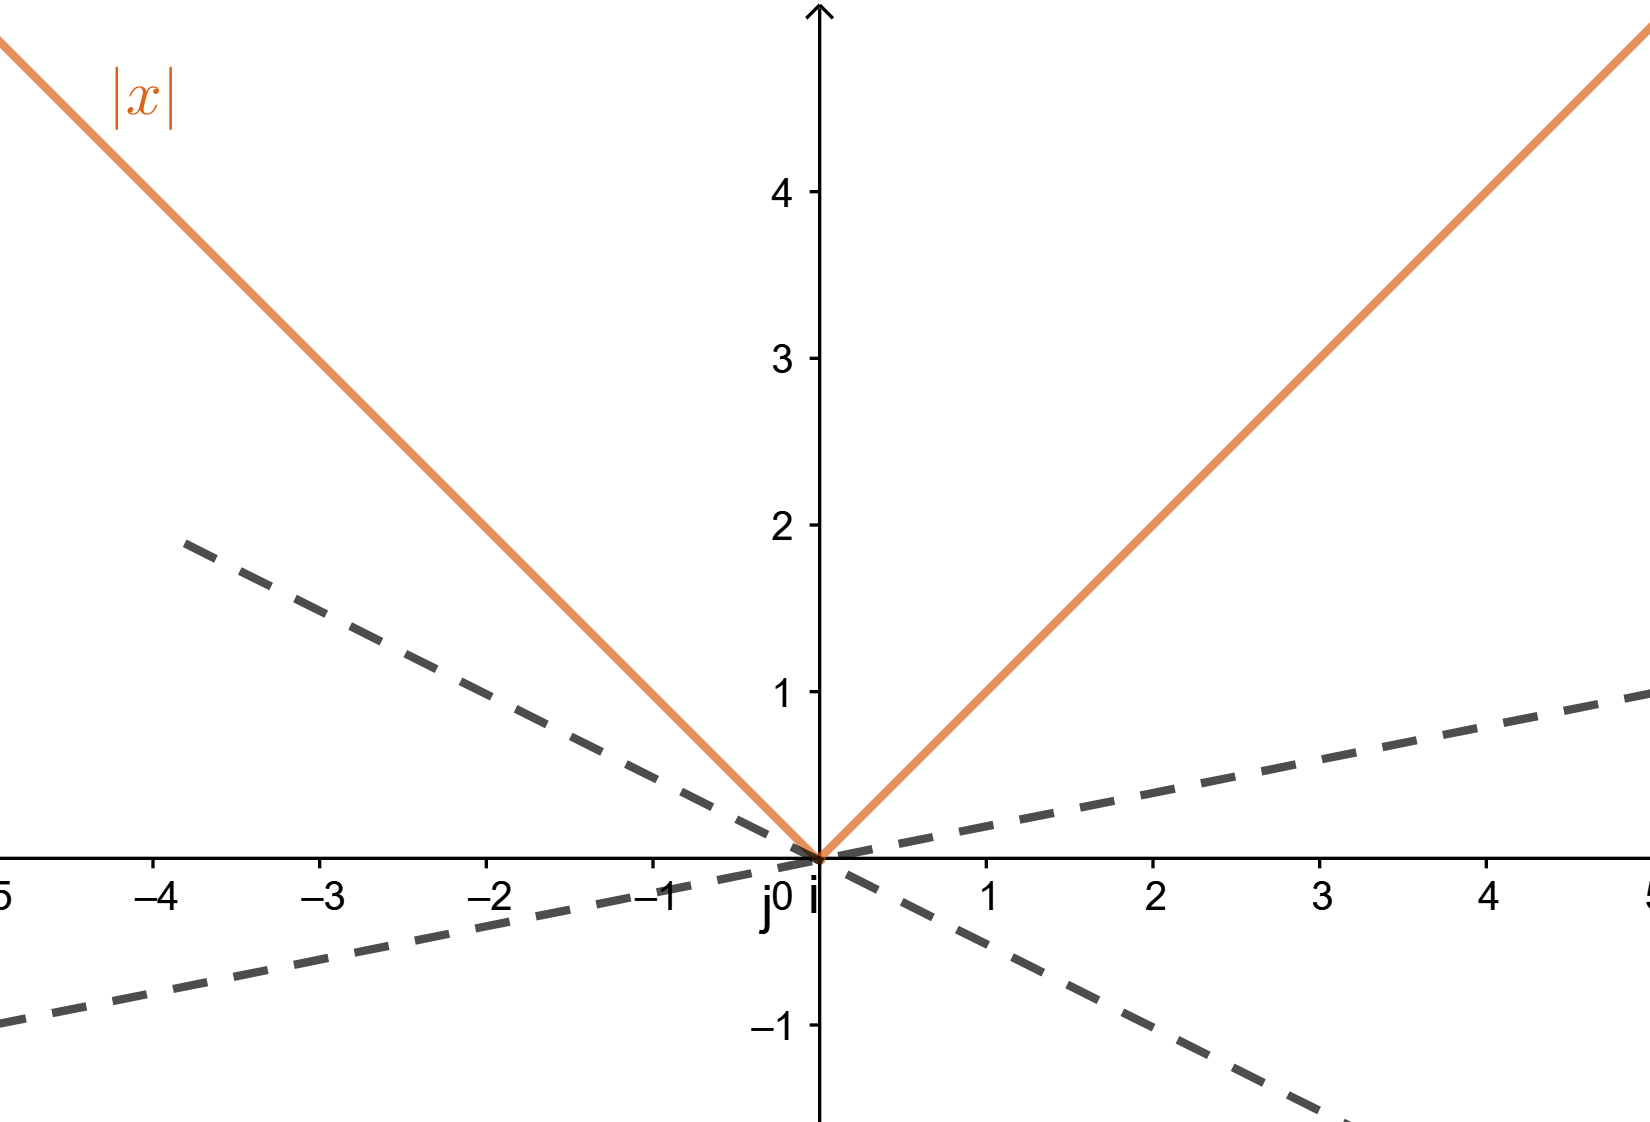
\includegraphics[width=8cm]{hinh_chuong4_algorithm/part5_subgradient_abs.png}
\caption{Bất cứ giá trị nào thuộc $[-1,1]$ đều là subgradient của hàm $f(x)=|x|$ tại điểm $x=0$.}
\end{figure}

\begin{figure}
\centering
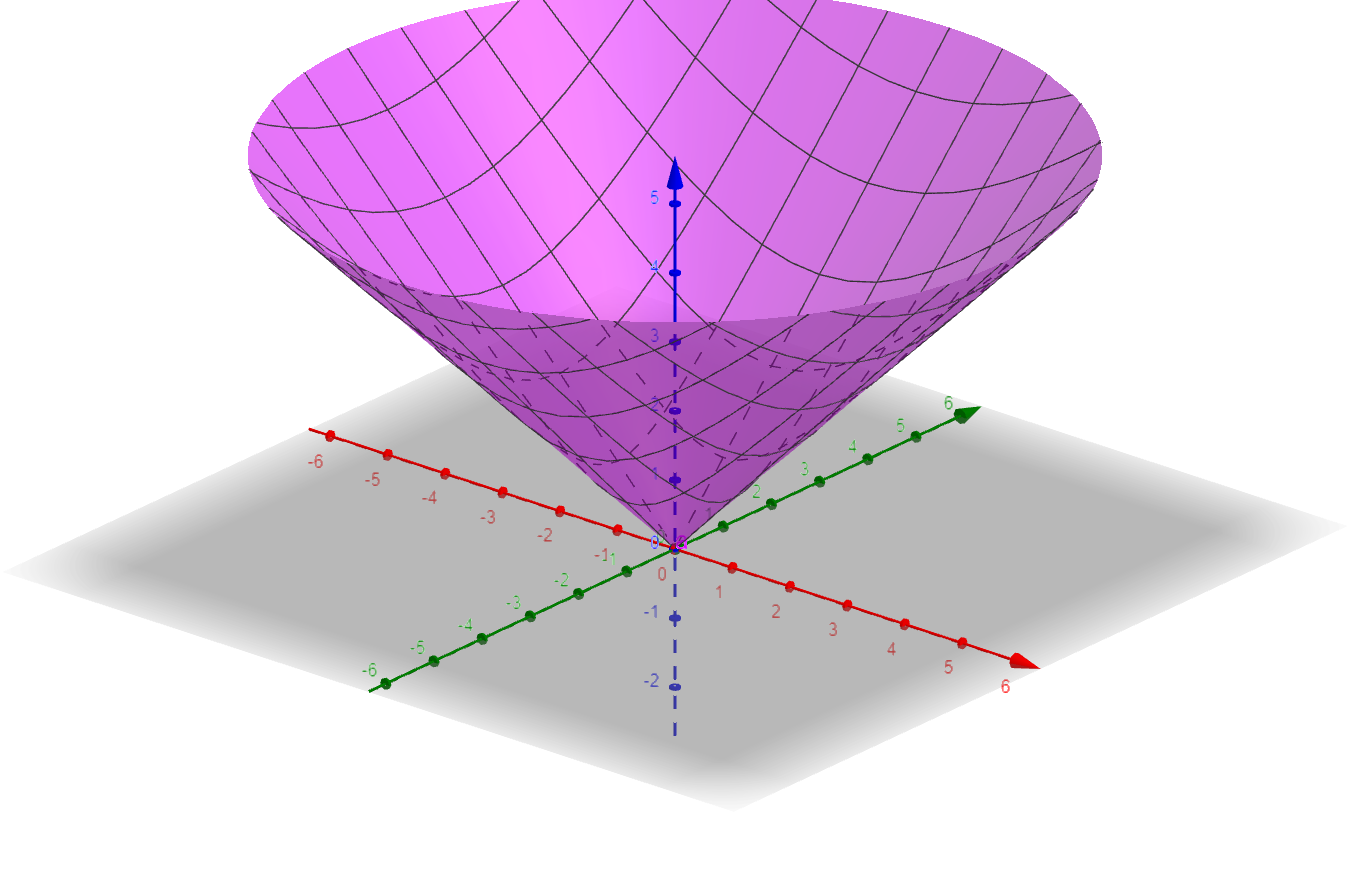
\includegraphics[width=8cm]{hinh_chuong4_algorithm/part5_subgradient_norm2.png}
\end{figure}

\begin{figure}
\centering
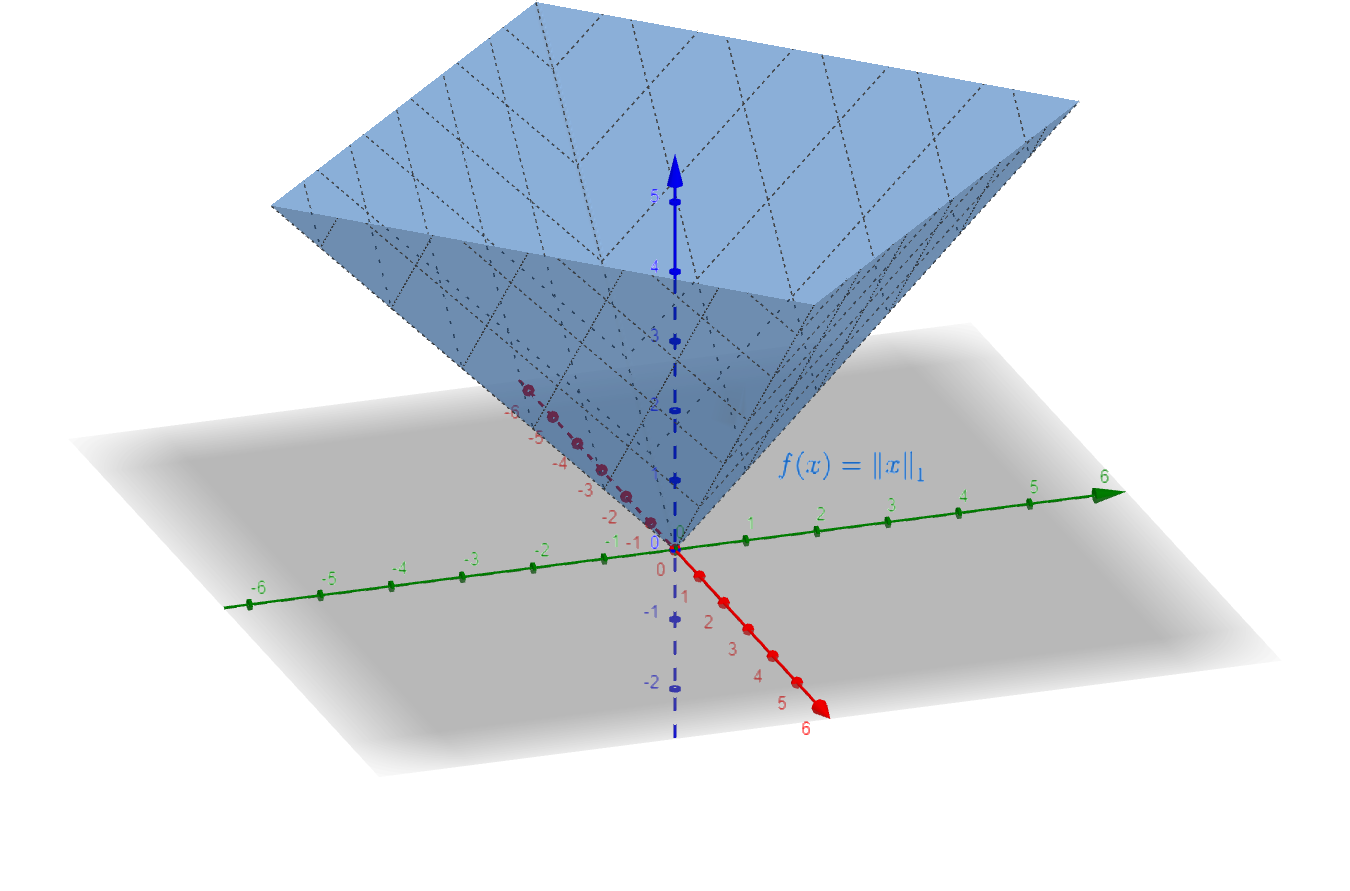
\includegraphics[width=8cm]{hinh_chuong4_algorithm/part5_subgradient_norm1.png}
\end{figure}


\subsection{Phương pháp subgradient}


Phương pháp subgradient rất tương tự như phương pháp gradient descent, nhưng thay vì cập nhật dùng gradient thì ta dùng subgradient:
\begin{align*}
x^{(k)} = x^{(k-1)} - t_k \nabla g^{(k-1)}, k = 1, 2, 3, \ldots
\end{align*}
trong đó $g^{(k-1)} \in \partial f(x^{(k-1)})$ là bất cứ subgradient nào của $f$ tại $x^{(k-1)}$.

\subsubsection{Tính chất hội tụ của phương pháp subgradient}

Định nghĩa giá tri $f(x_{best}^{(k)})$ tại bước lặp thứ $k$.
\begin{align*}
f_{best}^{(k)}=\min_{i=0,\ldots, k} f(x^{(i)}).
\end{align*}
Ta có thể tính $f_{best}^{(k)} = \min(f_{best}^{(k-1)}, f(x^{(k)})$.

Phương pháp subgradient được xem là hội tụ vì dãy $f_{best}^{(k)}$ hội tụ.
Lưu ý, phương pháp subgradient không phải là một phương pháp giảm dần (descent method).

\subsubsection{Một số cách chọn step size}
Một số kiểu step size áp dụng cho phương pháp subgradient:
\begin{itemize}
\item Step sizes hằng số: $t_k = t$
\item Diminishing step size: 
\begin{align*}
\sum_{k=1}^{\infty} t_k^2 < \infty, \quad \sum_{k=1}^{\infty} t_k =\infty,
\end{align*}
ví dụ $t_k = a/(b+k), a>0, b>0$.
%\item Nonsummable diminishing step size:
%\begin{align*}
%\lim_{k \rightarrow \infty} t_k =0 , \quad \sum_{k=1}^{\infty} t_k =\infty,
%\end{align*}
%ví dụ $t_k = a/\sqrt{k}, a>0$.
\end{itemize}

Nếu chọn step size hằng số thì $f_{best}^{(k)}$ hội tụ trong một lân cận $\epsilon$ của giá trị tối ưu.
Còn nếu chọn diminishing step size như $1/k$ thì $f_{best}^{(k)}$ hội tụ về chính xác giá trị tối ưu.

Cụ thể là, nếu hàm $f$ là Lipschitz continuous với hằng số $G >0$, tức là $\|f(x)-f(y)\| \leq G \|x-y\|$ với mọi $x,y$ thuộc miền xác định của $f$,
\begin{align*}
f(x_{best}^{(k)}) - f^* \leq \frac{R^2 + G^2 \sum_{i=1}^k t_i^2}{2\sum_{i=1}^k t_i}, 
\end{align*}
trong đó $R$ là một hằng số phụ thuộc vào điểm khởi tạo.
\begin{itemize}
\item Nếu chọn step size hằng số thì 
\begin{align*}
\lim_{k \rightarrow \infty} f(x_{best}^{(k)}) \leq f^* + G^2 t/2.
\end{align*}
$f_{best}^{(k)} - f^*$ hội tụ đến $G^2 t/2$.
\item Nếu chọn diminishing step sizes, 
\begin{align*}
\lim_{k \rightarrow \infty} f(x_{best}^{(k)}) = f^*.
\end{align*}
\end{itemize}


\subsection{Phương pháp subgradient áp dụng cho logistic regression với \textbf{$\ell_1$-norm regularization}}
Xét bài toán phân hai lớp logistic regression với \textbf{$\ell_1$-norm regularization} (LASSO) có dạng như sau:
\begin{align*}
\mathrm{max.~} J(w) &= \frac{1}{N}\sum_{i=1}^N y_i x_i^T w - \log (1 + e^{ x_i^T w}) - \lambda \|w\|_1,
\end{align*}
trong đó $x_i, y_i$ là vector đặc tính và nhãn của mẫu dữ liệu thứ $i$. 
(Xem logistic regression trong phần ứng dụng.)

Lưu ý:
\begin{itemize}
\item $\lambda \|w\|_1 = \sum_{j=1}^D w_j$ trong đó $D$ là số đặc tính của tập dữ liệu.
\end{itemize}

Đặt $J_i(w) = y_i x_i^T w - \log (1 + e^{ x_i^T w})$, ta có gradient của $J_i(w)$:
\begin{align*}
\nabla J_i(w) & = y_i x_i - \frac{e^{x_i^T w}}{1 + e^{x_i^T w}} * x_i \\
		& = (y_i - \sigma_i)x_i,
\end{align*}
trong đó  $\sigma_i = \frac{e^{x_i^T w}}{1 + e^{x_i^T w}}$.

Subgradient của regularization được chọn theo \eqref{eq:subgradient-norm1}:
\begin{align*}
\partial \lambda \|w\|_1 = \lambda \mathrm{sign}(w),
\end{align*}
trong đó, $\mathrm{sign}(w)_i = 1$ nếu $w_i > 0$, $\mathrm{sign}(w)_i = -1$ nếu $w_i < 0$ và $\mathrm{sign}(w)_i = 0$ nếu $w_i = 0$.

Do đó ta có
\begin{align*}
\partial J(w) & = \sum_{i=1}^N (y_i - \sigma_i)x_i - \lambda \mathrm{sign}(w).
\end{align*}
trong đó  $\sigma_i = \frac{e^{x_i^T w}}{1 + e^{x_i^T w}}$.
 
Giải thuật \textbf{subgradient} áp dụng cho logistic regression có dạng như sau:
\begin{algorithm}[H]
%\begin{algorithmic}[1]
khởi tạo $w$;\\
\textbf{repeat} 
\begin{enumerate}
\item chọn step size $t$.
\item Cập nhật: 
\begin{align*}
w := w + t \frac{1}{N}\sum_{i=1}^N \Big((y_i - \sigma_i)x_i - \lambda \mathrm{sign}(w) \Big)
\end{align*}
\end{enumerate}
\textbf{until} hội tụ. 
\caption{Giải thuật subgradient gradient áp dụng cho logistic regression.}
\label{alg:subgradient_logistic}
%\end{algorithmic}
\end{algorithm}

%\begin{algorithm}[H]
%\begin{algorithmic}[1]
%\STATE khởi tạo $w$;\\
%\REPEAT
%\STATE chọn step size $t$;
%\STATE cập nhật $w$: 
%\begin{align*}
%w := w + t \Big(\frac{1}{N}\sum_{i=1}^N (y_i - \sigma_i)x_i - \lambda \mathrm{sign}(w) \Big);
%\end{align*}
%\UNTIL{hội tụ.} 
%\end{algorithmic}
%\caption{Giải thuật subgradient áp dụng cho logistic regression.}
%\label{alg:subgradient_logistic}
%\end{algorithm}

\textbf{Lưu ý}, bài toán tối ưu là bài toán tìm cực đại hàm lõm, do đó cập nhật phải có dạng
\begin{align}
w := w + t \nabla J(w).
\label{eq:grad_ascent}
\end{align}

\begin{figure}[h]
	\centering
	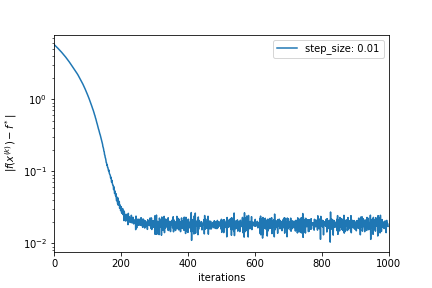
\includegraphics[width=8cm]{hinh_chuong4_algorithm/part5_logistic-regression_synthetic_subgradient_norm1_fix-s0.01.png}
	\caption{Giải thuật subgradient với fix step size \lstinline{step_size = 0.01}.}
	\label{fig:descent}	
\end{figure}

\begin{figure}[h]
	\centering
	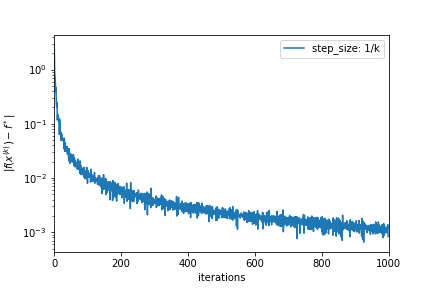
\includegraphics[width=8cm]{hinh_chuong4_algorithm/part5_logistic-regression_synthetic_subgradient_norm1_diminising-s1.png}
	\caption{Giải thuật subgradient với diminishing step size \lstinline{step_size = 1/k}. Độ chính xác nếu dùng diminishing step size cao hơn so với dùng fix step size.}
	\label{fig:descent}	
\end{figure}



\newpage
\section{PROXIMAL GRADIENT METHOD}
Các phương pháp proximal có thể được dùng cho các bài toán có tập dữ liệu lớn với nhiều thuộc tính. Các phương pháp này đều có sử dụng biến đổi proximal. Khác với các phương pháp gradient descent, Newton, phương pháp proximal dùng trong trường hợp hàm mục tiêu không khả vi, tuy nhiên tốc độ hội tụ lại tốt như gradient descent và nhanh hơn phương pháp sugradient.

\subsection{Phép biến đổi proximal}
Cho hàm số $f: \mathbb{R}^n \rightarrow \mathbb{R}$ lồi.
Phép biến đổi proximal (tiếng Anh là proximal operator) tương ứng với hàm $f$ được định nghĩa
\begin{align*}
\textrm{prox}_f (v) = \textrm{argmin}_x \big(f(x) + \frac{1}{2} \| x - v \|^2_2 \big).
\end{align*}
Trong một số ứng dụng, hàm $f$ được nhân với một tham số $\lambda >0$, ta có
\begin{align*}
\textrm{prox}_{\lambda f} (v) = \textrm{argmin}_x \big(f(x) + \frac{1}{2\lambda} \| x - v \|^2_2 \big).
\end{align*}

Phép biến đổi proximal có thể được xem là biến đổi điểm $x$ về một điểm $v$ gần điểm cực tiểu của $f(x)$ nhưng vẫn gần với điểm $x$. Tham số $\lambda$ có ý nghĩa là trọng số điều chỉnh mối tương quan giữa hai đại lượng này. 
(Chữ proximity trong tiếng Anh có nghĩa là gần, trong lân cận.)


\subsubsection{Một số tính chất của proximal}

\begin{itemize}

\item \textbf{Tổng của các hàm tách biệt:}
 
Nếu hàm $f$ có dạng 
\begin{align*}
f(x,y) = g(x) + h(y),
\end{align*}
thì 
\begin{align*}
\textrm{prox}_f (v,w) = (\textrm{prox}_g(v), \textrm{prox}_h(w)).
\end{align*}
Như vậy đối với hàm có dạng tổng các hàm tách biệt, biến đổi proximal của hàm đó tương ứng với biến đổi proximal với từng hàm riêng biệt.

Trường hợp mở rộng, nếu $f(x) = \sum_{i=1}^n f_i(x_i)$, trong đó, $x = (x_1,\ldots,x_n)$ ta có 
\begin{align*}
(\textrm{prox}_f (v))_i = \textrm{prox}_{f_i}(v_i).
\end{align*}

\item \textbf{Fix point:}
$x^*$ là điểm cực tiểu của $f(x)$ nếu và chỉ nếu
\begin{align*}
x^* = \textrm{prox}_f(x).
\end{align*}

\item \textbf{Các tính chất khác:}

\noindent Nếu hàm $f(x) = a g(x) + b, a>0$ thì
\begin{align*}
\textrm{prox}_{\lambda f} (v) = \textrm{prox}_{a \lambda g}(v).
\end{align*}

\noindent Nếu hàm $f(x) = g(ax + b), a \neq 0$ thì 
\begin{align*}
\textrm{prox}_{\lambda f} (v) = \frac{1}{a} \big(\textrm{prox}_{a^2 \lambda g}(av + b) - b\big).
\end{align*}

\noindent Nếu $f(x) = g(x) + a^Tx + b$ thì
\begin{align*}
\textrm{prox}_{\lambda f} (v) = \textrm{prox}_{\lambda g}(v - \lambda a).
\end{align*}
\end{itemize}

\subsection{Phương pháp proximal gradient}
Xét hàm số $f: \mathbb{R}^n \rightarrow \mathbb{R}$ có dạng
\begin{align*}
\min f(x) = g(x) + h(x),
\end{align*} 
trong đó $g$ là hàm lồi và khả vi, $h$ là hàm lồi và có thể không khả vi. 
Do đó, hàm $f$ có thể không phải là hàm khả vi.

Ta có thể áp dụng phương pháp subgradient để tìm cực tiểu hàm $f$. Phương pháp subgradient hội tụ với diminishing step size, ví dụ step size $t_k = a / k$. Tốc độ hội tụ là $O(1/\epsilon^2)$ hay $O(1/\sqrt{k})$. Trong phần này, tôi trình bày về phương pháp proximal gradient áp dụng cho bài toán có tốc độ hội tụ như gradient descent.

Nếu như $f$ khả vi, phương pháp gradient descent cập nhật theo xấp xỉ bậc 2 hàm $f$ xung quanh điểm $x^k$:
\begin{align*}
x^{k+1} &= \textrm{argmin}_z \bar{f}_t(z) = \textrm{argmin}_z f(x^k) + \nabla f(x^k)^T (z - x^k) + \frac{1}{2t} \| z - x^k \|^2_2 \\
		& = x^k - t . \nabla f(x^k).
\end{align*}

Trong trường hợp, hàm $f$ không khả vi do $h$ không khả vi, phương pháp \textbf{proximal gradient} thực hiện xấp xỉ hàm $g$ như sau:
\begin{align*}
x^{k+1} & = \textrm{argmin}_z \bar{g}_t(z) + h(z) \\
		& = \textrm{argmin}_z f(x^k) + \nabla f(x^k)^T (z - x^k) + \frac{1}{2t} \| z - x^k \|^2_2 + h(z)\\
		& = \textrm{argmin}_z \frac{1}{2t} \| z - (x^k - t . \nabla g(x^k))\|_2^2 + h(z) \\
		& = \textrm{prox}_{t_k h}(x^{(k)} - t_k . \nabla g(x^{(k)})).
\end{align*}

Theo định nghĩa của biến đổi proximal bên trên, cập nhật trong \textbf{phương pháp proximal gradient} có dạng
\begin{align*}
x^{(k+1)} = \textrm{prox}_{t_k h}(x^{(k)} - t_k . \nabla g(x^{(k)})), k=1, 2, \ldots
\end{align*}

Giải thuật proximal gradient được mô tả như sau:
\begin{algorithm}[H]
%\begin{algorithmic}[1]
khởi tạo $x^{(0)}$;\\
cho $k = 0,1,\ldots$\\
\textbf{repeat} 
\begin{enumerate}
\item \textbf{Gradient descent}: $y^{(k)} = x^{(k)} - t_k . \nabla g(x^{(k)})$
\item \textbf{Proximal}: $x^{(k+1)} = \mathrm{prox}_{t_k h}(y^{(k)} =  \textrm{argmin}_z \frac{1}{2t_k} \| z - y^{(k)}\|_2^2 + h(z)$
\end{enumerate}
\textbf{until} hội tụ. 
\caption{Phương pháp proximal gradient.}
\label{alg:proximal}
%\end{algorithmic}
\end{algorithm}

Trong trường hợp proximal của hàm $h$ có tính toán đơn giản, ví dụ như có dạng công thức tường minh thì độ phức tạp trong mỗi vòng lặp chủ yếu là ở bước tính gradient của hàm $g$, bằng với độ phức tạp của giải thuật gradient descent.

Trong thực tế, vài hàm quan trọng $h$ có biến đổi proximal dạng công thức tường minh.
Sau đây trình bày một ví dụ về phương pháp proximal gradient dùng cho LASSO.


\subsubsection*{Tốc độ hội tụ của phương pháp proximal gradient}
Cho hàm $f(x) = g(x) + h(x)$. Giả sử rằng
\begin{itemize}
\item $g$ là hàm lồi, khả vi trên $\mathbb{R}^n$, và hàm $\nabla g$ là Lipschitz continuous với tham số $L>0$;
\item $h$ là hàm lồi và biến đổi $\mathrm{prox}_t(x) = \mathrm{argmin}_z \{ \frac{1}{2t}\| x - z \|_2^2  + h(z) \}$ có thể tính được dễ dàng.
\end{itemize}

Ta có giải thuật proximal gradient với step size hằng số $t \leq 1/L$ thoả mãn
\begin{align*}
f(x^{(k)}) - f^* \leq \frac{\|x^{(0)} - x^*\|_2^2}{2tk}.
\end{align*}
Nếu sử dụng step size tìm bởi backtracking line search với $t = \beta / L$ thì kết quả trên vẫn không đổi.

Công thức trên cho thấy \textbf{giải thuật proximal gradient hội tụ theo $O(1/k)$ hay $O(1/\epsilon)$}.
Cùng tốc độ hội tụ với gradient descent.


\subsection{Giải thuật Iterative Shrinkage-Thresholding Algorithm (ISTA) cho LASSO}
LASSO (least absolute shrinkage and selection operator) có nghĩa là tìm nghiệm với $\ell_1$-norm regularization. (Bạn đọc xem định nghĩa về norm trong phần \textit{hàm convex}.)
LASSO được định nghĩa đầu tiên cho hồi quy tuyến tính. Sau đó nó được mở rộng dùng cho các bài toán khác.
Sử dụng LASSO giúp thể hiện được những đặc tính chính trong tập dữ liệu. Các đặc tính không quan trọng có trọng số bằng 0.
Giải thuật Iterative Shrinkage-Thresholding Algorithm (ISTA) chính là áp dụng phương pháp proximal gradient cho LASSO.

Gọi $d = \begin{bmatrix}
d_1 \\ d_2 \\ \ldots \\ d_n
\end{bmatrix} \in \mathbb{R}^n$ là số đặc tính của tập dữ liệu và ma trận $A = \begin{bmatrix}
a_1^T \\ a_2^T \\ \ldots \\ a_n^T
\end{bmatrix} \in \mathbb{R}^{n \times p}$, \\
bao gồm các vector $a_i = \begin{bmatrix}
a_{i1} \\ a_{i2} \\ \ldots \\ a_{ip}
\end{bmatrix} \in \mathbb{R}^p$ tương ứng với nhãn $d_i$.\\

Quy hoạch tuyến tính dùng LASSO được định nghĩa là bài toán tối ưu
\begin{align*}
\min_w f(w) = g(w) + h(w) = \frac{1}{2} \| Aw - d \|_2^2 + \lambda \|w\|_1.
\end{align*}

Giải thuật thực hiện có dạng:
\begin{algorithm}[H]
%\begin{algorithmic}[1]
khởi tạo $w^{(0)}$;\\
cho $k = 0,1,\ldots$\\
\textbf{repeat} 
\begin{enumerate}
\item \textcolor{blue}{Gradient descent}: $v^{(k)} =  w^{(k)} - t A^T (A w^{(k)} - d)$
\item \textcolor{blue}{Proximal}: $w^{(k + 1)} = \textrm{prox}_{\lambda t \|z\|_1}(v^{(k)}) =  \textrm{argmin}_z \frac{1}{2t} \| z - v^{(k)} \|_2^2 + \lambda \|z\|_1$.
\end{enumerate}
\textbf{until} hội tụ. 
\caption{Giải thuật Iterative Shrinkage-Thresholding Algorithm (ISTA) cho LASSO.}
\label{alg:ISTA}
%\end{algorithmic}
\end{algorithm}

Proximal cho $\ell_1$-norm được tính như sau: 
\begin{align*}
\textrm{prox}_{\lambda t \|z\|_1}(v^{(k)}) &=  \textrm{argmin}_z \frac{1}{2t} \| z - v^{(k)} \|_2^2 + \lambda \|z\|_1 \\
&  = \textrm{argmin}_{z} \sum_{i = 1}^p \frac{1}{2}(z_i - v_i^{(k)})^2 + \lambda t |z_i| \\
&  = \sum_{i = 1}^p \textrm{argmin}_{z_i} \frac{1}{2} (z_i - v_i^{(k)})^2 + \lambda t |z_i|,  i = 1, \ldots, p
\end{align*}
Áp dụng điều kiện đạt cực trị của một hàm tổng quát
\begin{align*}
z_i^* = \textrm{argmin}_{z_i} \frac{1}{2}(z_i - v_i^{(k)})^2 + \lambda t |z_i|,
\end{align*}
ta cần tìm $z_i$ sao cho $\partial \frac{1}{2}(z_i - v_i^{(k)})^2 + \lambda t |z_i| = 0$.

Ta đã biết subgradient của $|z_i|$:
\begin{align*}
\partial |z_i| = \begin{cases} 1, \textrm{ nếu } z_i > 0,\\
							-1, \textrm{ nếu } z_i < 0,\\ 
							[-1,1], \textrm{ nếu } z_i = 0.\end{cases}
\end{align*}
Do đó, nghiệm của $0 \in \partial (z_i - v_i^{(k)})^2 + \lambda |z_i|$ chính là phép biến đổi \textbf{soft-threshold}:
\begin{align*}
w^{(k+1)}_i = \begin{cases} v_i^{(k)} - \lambda t ~ & \textrm{ nếu } v_i^{(k)} > \lambda t \\ 
0 & \textrm{ nếu } -\lambda t \leq v_i^{(k)} \leq \lambda t\\
v_i^{(t)} + \lambda t ~ & \textrm{ nếu } v_i^{(k)} < -\lambda t. \end{cases}
\end{align*}

%\subsection{Thực hiện trên Python}
%Phần tiếp theo đây là chương trình python thực hiện giải thuật subgradient cho logistic regression với tập dữ liệu nhân tạo. Đối với các bài toán khác, ta cũng có thể theo cấu trúc tương tự. Điều quan trọng là ước lượng được subgradient tại mỗi vòng lặp.
%
%Trước tiên ta import các thư viện:
%\begin{lstlisting}[language=Python]
%import numpy as np
%import matplotlib.pyplot as plt
%\end{lstlisting}


\subsection{Phương pháp projected gradient descent}
Bây giờ xét bài toán tìm cực tiểu có ràng buộc:
\begin{align*}
\min_{x \in C} g(x),
\label{eq:constraint_prob}
\end{align*}
trong đó tập $C \in \mathbb{R}^n$ là tập lồi đóng.
Bài toán trên tương đương với bài toán
\begin{align}
\min_x g(x) + I_C (x),
\end{align}
trong đó $I_C$ là hàm indicator cho tập $C$,
\begin{align*}
I_C (x) = \begin{cases} 0 ~\mathrm{if}~ x \in C \\ \infty ~\mathrm{if}~ x \notin C \end{cases}.
\end{align*}

Ta có
\begin{align*}
\mathrm{prox}_{I_C}(x) &= \mathrm{argmin}_z \left( \frac{1}{2}\| x - z \|_2^2  + I_C (z) \right) \\
				& = \mathrm{argmin}_{z \in C} \frac{1}{2}\| x - z \|_2^2  \\
				& = P_C(x),
\end{align*}
chính là hình chiếu của $x$ lên tập $C$.

Do đó, nếu áp dụng phương pháp proximal gradient lên bài toán \eqref{eq:constraint_prob}, cập nhật sẽ có dạng: 
\begin{align*}
x^{(k+1)} = P_C (x^{(k)} - t \nabla g(x)).
\end{align*}
Tức là thực hiện cập nhật theo gradient descent thông thường, sau đó tìm hình chiếu lên tập $C$.

Giải thuật projected gradient descent được mô tả như sau:
\begin{algorithm}[H]
%\begin{algorithmic}[1]
khởi tạo $x^{(0)}$;\\
cho $k = 0,1,\ldots$\\
\textbf{repeat} 
\begin{enumerate}
\item Gradient descent: $v^{(k)} =  x^{(k)} - t \nabla g(x)$
\item Projection: $x^{(k + 1)} = P_C(v^{(k)})$
\end{enumerate}
\textbf{until} hội tụ. 
\caption{Giải thuật projected gradient descent.}
\label{alg:projectedGD}
%\end{algorithmic}
\end{algorithm}

\textbf{Lưu ý}: Thông thường thì tìm hình chiếu lên một tập $C$ là một bài toán tối ưu phức tạp đòi hỏi giải thuật lặp để tìm nghiệm. Tuy nhiên với một số tập $C$ dạng đơn giản thì ta có thể dễ dàng tìm hình chiếu. Ví dụ:
\begin{itemize}
\item $C = \mathbb{R}^n_+ = \{x \in \mathbb{R}^n | x \geq 0 \}$: $P_{C}(x)\ = x_+$, 
\begin{align*}
(x_+)_i = \max(0, x_i). 
\end{align*}

\item dạng box $C = \{ x | l \leq x \leq u \}$:
\begin{align*}
(P_C(x))_i = \begin{cases} l_i \textrm{ nếu } x_i \leq l_i \\ 
							x_i \textrm{ nếu } l_i \leq x_i \leq u_i \\
							u_i \textrm{ nếu } x_i \geq u_i. \end{cases} 
\end{align*}

\item $C = \{ x \in \mathbb{R}^n | Ax = b\}$, trong đó $A \in \mathbb{R}^{m \times n}$:
\begin{align*}
P_C (x) = x - A^{\dagger}(Ax - b),
\end{align*}
trong đó $A^{\dagger} = A^T(AA^T)^{-1}$, ma trận Moore-Penrose pseudoinverse của $A$.
\end{itemize}





\begin{thebibliography}{8}
\bibitem{boyd}
Boyd, Stephen, Stephen P. Boyd, and Lieven Vandenberghe. Convex optimization. Cambridge university press, 2004.

\bibitem{cmulectures}
Convex optimization lectures. Available at www.stat.cmu.edu/$\sim$ryantibs/convexopt/.
\end{thebibliography}
\end{document}
